\section{Results}
\label{sec:Results}

The shapes of the distributions of the truth and reco leading jet \pt~observables are very similar, but not identical (especially in the first bins), as illustrated in Figure~\ref{fig:jetPt} for the training set (left) and for the testing set (right).

\begin{figure}[h]
  \centering
  \includegraphics[width=0.49\textwidth]{../output_20GeV/NN_plot1D_train_jetPt_truth_reco.pdf}
  \includegraphics[width=0.49\textwidth]{../output_20GeV/NN_plot1D_test_jetPt_truth_reco.pdf}
  \caption{Overlay with ratio pad of the truth and reco leading jet \pt. Train and Test.}
  \label{fig:jetPt}
\end{figure}

Two figures of merit are used to optimise the NN hyper-parameters. The accuracy: the larger, the better (left: old NN; right: new NN). The loss (error) value: the smaller, the better (left: old NN; right: new NN). The overlaid train and test are very similar, which confirms the NNs are not overtrained.

\begin{figure}[h]
  \centering
  \includegraphics[width=0.49\textwidth]{../output_20GeV/NN_plot1D_optionTrainTest_accuracy_NN_l_A1_k_8_e_150_b_1000.pdf}
  \includegraphics[width=0.49\textwidth]{../output_20GeV/NN_plot1D_optionTrainTest_accuracy_NN_l_B3_k_4_e_150_b_200.pdf}
  \caption{Overlay with ratio pad of the truth and reco leading jet \pt. Old and new NN.}
  \label{fig:accuracyTrainTest}
\end{figure}

\begin{figure}[h]
  \centering
  \includegraphics[width=0.49\textwidth]{../output_20GeV/NN_plot1D_optionTrainTest_loss_NN_l_A1_k_8_e_150_b_1000.pdf}
  \includegraphics[width=0.49\textwidth]{../output_20GeV/NN_plot1D_optionTrainTest_loss_NN_l_B3_k_4_e_150_b_200.pdf}
  \caption{Overlay with ratio pad of the truth and reco leading jet \pt. Old and new NN.}
  \label{fig:lossTrainTest}
\end{figure}

Overlaying the two NN architectures, the old and new. The accuracy is the larger, the better.

\begin{figure}[h]
  \centering
  \includegraphics[width=0.49\textwidth]{../output_20GeV/NN_plot1D_train_accuracy_NN_final.pdf}
  \includegraphics[width=0.49\textwidth]{../output_20GeV/NN_plot1D_test_accuracy_NN_final.pdf}
  \caption{Overlay with old and new NN for the accuracy value (the smaller the better).}
  \label{fig:accuracyOldNew}
\end{figure}

\begin{figure}[h]
  \centering
  \includegraphics[width=0.49\textwidth]{../output_20GeV/NN_plot1D_train_loss_NN_final.pdf}
  \includegraphics[width=0.49\textwidth]{../output_20GeV/NN_plot1D_test_loss_NN_final.pdf}
  \caption{Overlay with old and new NN for the loss value (the larger the better). Train and test.}
  \label{fig:lossOldNew}
\end{figure}

The jet pt distribution as the index of the jet pt bin. True output (generated, truth) vs input (reconstructed). Used in traditional unfolding.

\begin{figure}[h]
  \centering
  \includegraphics[width=0.49\textwidth]{../output_20GeV/NN_plot1D_train_jetPtBin_NN_noTrained.pdf}
  \includegraphics[width=0.49\textwidth]{../output_20GeV/NN_plot1D_test_jetPtBin_NN_noTrained.pdf}
  \caption{Overlay ?. Train and test.}
  \label{fig:ptIndexNoTrained}
\end{figure}

The true output vs the predicted unfolded output by each NN architecture. The new NN architecture is closer to the true output than the old one.

\begin{figure}[h]
  \centering
  \includegraphics[width=0.49\textwidth]{../output_20GeV/NN_plot1D_train_jetPtBin_NN_final.pdf}
  \includegraphics[width=0.49\textwidth]{../output_20GeV/NN_plot1D_test_jetPtBin_NN_final.pdf}
  \caption{Overlay ?. Train and test.}
  \label{fig:ptIndexFinal}
\end{figure}

The predicted NN output minus the true output.  Both outputs are integers, representing bin indices. Therefore the difference is also an integer. The greater the count at zero difference, the better.  Top: train, bottom: test. Left to right, bin widths of 10, 20, 50, 100 GeV. The smaller the binWidth, the better is the new NN architecture relative to the old one.

\begin{figure}[h]
  \centering
  \includegraphics[width=0.49\textwidth]{../output_10GeV/NN_plot1D_train_outputPredictedMinusTrue_NN_final.pdf}
  \includegraphics[width=0.49\textwidth]{../output_10GeV/NN_plot1D_test_outputPredictedMinusTrue_NN_final.pdf}\\
  \includegraphics[width=0.49\textwidth]{../output_20GeV/NN_plot1D_train_outputPredictedMinusTrue_NN_final.pdf}
  \includegraphics[width=0.49\textwidth]{../output_20GeV/NN_plot1D_test_outputPredictedMinusTrue_NN_final.pdf}\\
  \includegraphics[width=0.49\textwidth]{../output_50GeV/NN_plot1D_train_outputPredictedMinusTrue_NN_final.pdf}
  \includegraphics[width=0.49\textwidth]{../output_50GeV/NN_plot1D_test_outputPredictedMinusTrue_NN_final.pdf}\\
  \includegraphics[width=0.49\textwidth]{../output_100GeV/NN_plot1D_train_outputPredictedMinusTrue_NN_final.pdf}
  \includegraphics[width=0.49\textwidth]{../output_100GeV/NN_plot1D_test_outputPredictedMinusTrue_NN_final.pdf}\\
  \caption{Overlay ?. Train and test.}
  \label{fig:binIndexPredictedMinusTruel}
\end{figure}

The 2D histogram migration matrix of the index of the jet pt. The closer to a diagonal matrix, the better.

\begin{figure}[h]
  \centering
  \includegraphics[width=0.49\textwidth]{../output_20GeV/NN_plot2D_train_outputTrue_input.pdf}
  \includegraphics[width=0.49\textwidth]{../output_20GeV/NN_plot2D_test_outputTrue_input.pdf}\\
  \includegraphics[width=0.49\textwidth]{../output_20GeV/NN_plot2D_train_outputTrue_outputPredicted_NN_l_A1_k_8_e_150_b_1000.pdf}
  \includegraphics[width=0.49\textwidth]{../output_20GeV/NN_plot2D_test_outputTrue_outputPredicted_NN_l_A1_k_8_e_150_b_1000.pdf}\\
  \includegraphics[width=0.49\textwidth]{../output_20GeV/NN_plot2D_train_outputTrue_outputPredicted_NN_l_B3_k_4_e_150_b_200.pdf}
  \includegraphics[width=0.49\textwidth]{../output_20GeV/NN_plot2D_test_outputTrue_outputPredicted_NN_l_B3_k_4_e_150_b_200.pdf}\\
  \caption{Overlay ?. Train and test.}
  \label{fig:2DMigrationMatrix}
\end{figure}


The solution is using these NN architectures.

\begin{figure}[h]
  \centering
  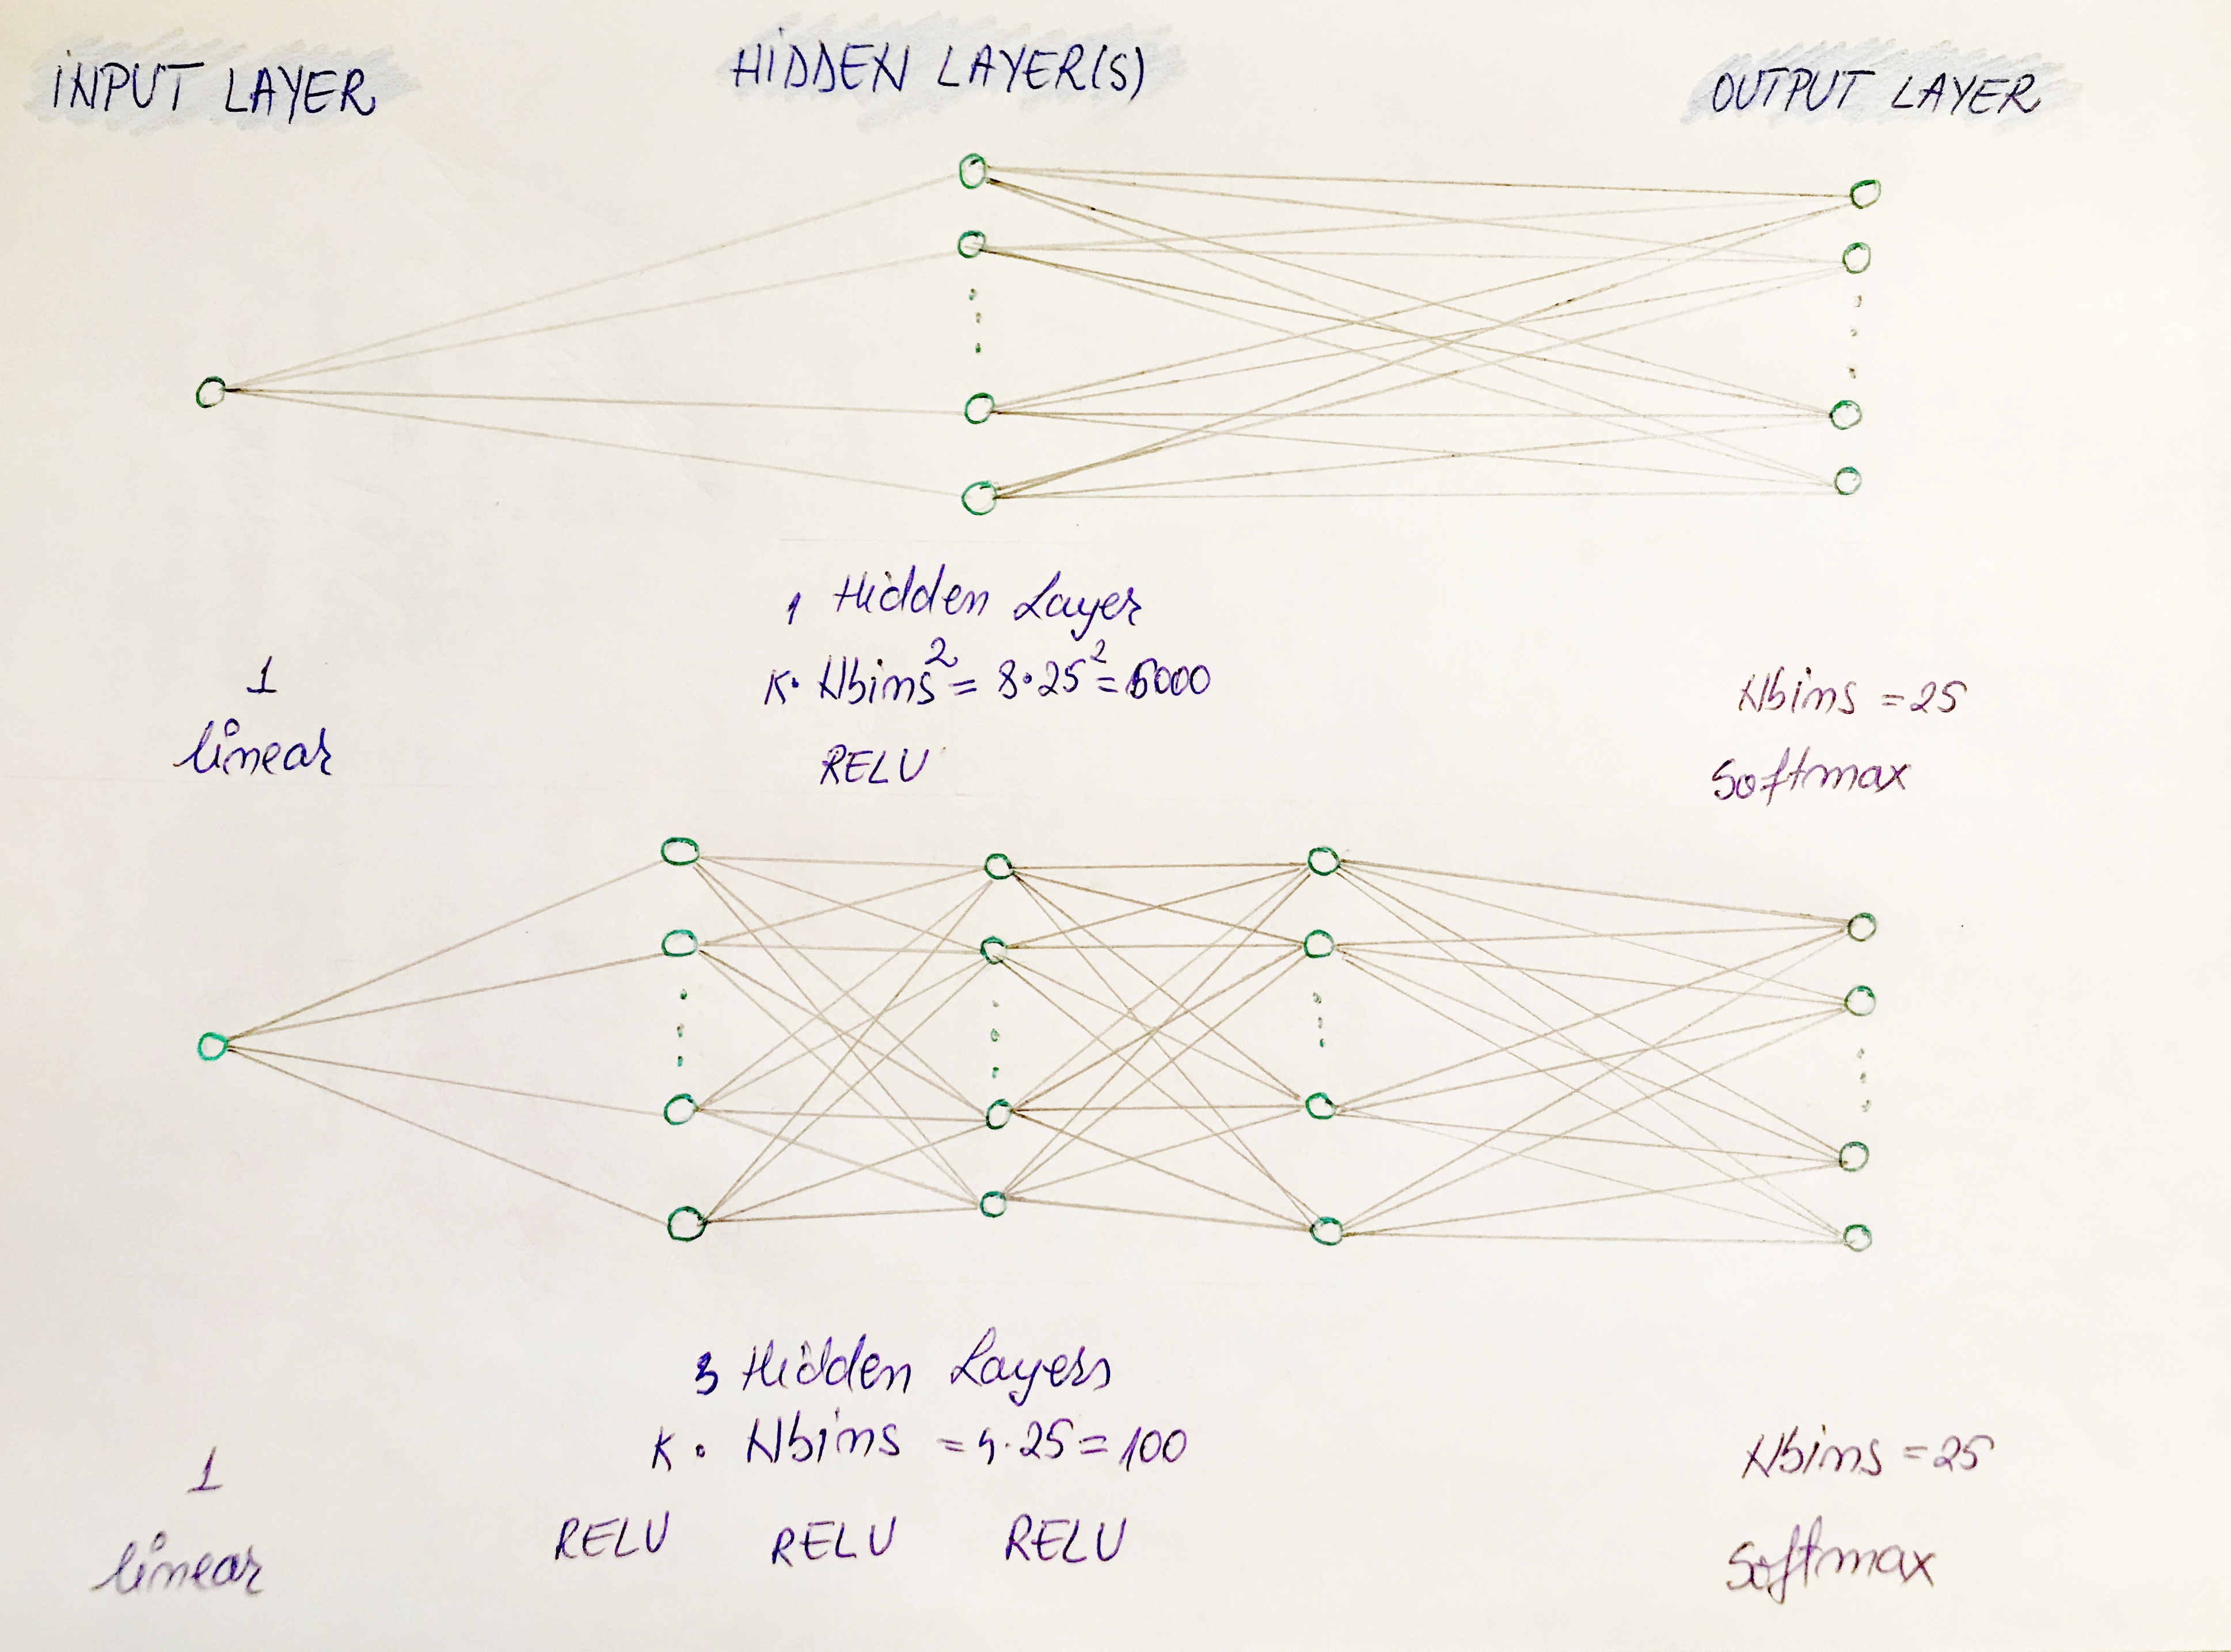
\includegraphics[width=0.49\textwidth]{../presentation/plots/NNArchitecture.jpg}
  \caption{Diagram of the physics problem.}
  \label{fig:NNArchitecture}
\end{figure}

 Fine tuned the NN hyper parameters for our ROOT data sample. One NN training is the first step of the iterative unfolding procedure. {Summary of the physics and NN choices. 

One file with 43076 events (and leading jets). Half (21538) in training, half in testing. jet pt: range=0-500 GeV, bin width=20 GeV, number of bins = 500/20 = 25.  Chose the NN training hyper-parameters by changing one at a time while keeping the other constant, and choosing those with largest accuracy and smallest loss values. 

\begin{table}[h!]
  \resizebox{\textwidth}{!}{
    \begin{tabular}{|l|l|l|} % <-- Alignments: 1st column left, 2nd middle and 3rd right, with vertical lines in between
      \hline
      \textbf{Choice} & \textbf{Old NN (toy data example)} & \textbf{New NN (my best choice)}\\
      \hline
      number of nodes per input layer & 1 & 1 \\
      number of nodes per output layer & ${\rm Nbins}=25$ & ${\rm Nbins}=25$ \\
      Number of hidden layers & 1 & 3 \\
      ${\rm k}$ & 8 & 4 \\
      Number of nodes per layer & ${\rm k}\cdot {\rm Nbins}^2=5000$ & ${\rm k}\cdot {\rm Nbins}=100$ \\
      activation function input & linear & linear \\
      activation function hidden & ReLU & ReLU \\
      activation function output & softmax & softmax \\
      batch size & 1000 & 200 \\
      number of epochs & 150 & 150 \\
      \hline
    \end{tabular}
  }
\caption {NN architecture and hyper-parameters comparing for the old NN, suggested in the toy data paper, and the new NN, from the optimisation of this study.}
\end{table}
